To get a better intuition for the different definitions of a corner, we'll use them for some things that are not directly related to solving LPs.

\subsection*{Convex Hulls}

\begin{Def}(Convex Hull) Let $x_1,\ldots,x_k$ be some vectors in $\R^n$. The convex hull of these vectors is
\[\mbox{CH}(\{x_1,\ldots,x_k\}) = \left\{\sum _{i=1}^k \lambda_i x_i \left| \sum_{i=1}^k \lambda_i =1,\ \lambda_i\geq 0\right.\right\}\]
\end{Def}

Here we generalise the notion of convex combination to use more than two points. Intuitively if we have a bunch of points in 2D we get all the points that lie within the polygon that is spanned by the points on the CH, see figure \ref{Fig:convexHull}.

\begin{figure}[hbt]
\begin{center}
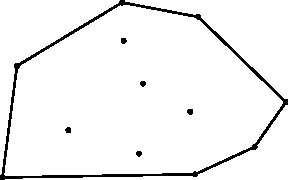
\includegraphics{./images/convex_hull.pdf}
\end{center}
\caption{The convex hull of a set of points}
\label{Fig:convexHull}
\end{figure}

This definition allows us to come up with a different definition of a polyhedron. In contrast to definition \ref{Def:polyhedron} the convex hull definition allows us to have a more geometric view of the problem.

\begin{Def}[Bounded Polyhedra] A bounded polyhedron lies within a finite bounding box, see figure \ref{Fig:bounded_unbounded}. More formally

\[\forall x\in P,d\in \R^n, \forall \lambda > 0: x+\lambda d \not \in P\]

For any line from a point inside the polyhedron we eventually leave the polyhedron
\end{Def}

\begin{figure}[hbt]
\begin{center}
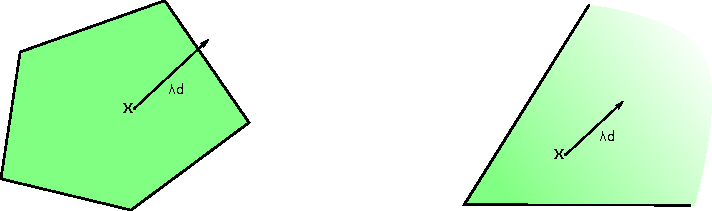
\includegraphics{./images/bounded_unbounded.pdf}
\end{center}
\caption{A bounded (left) and an unbounded (right) polyhedron}
\label{Fig:bounded_unbounded}
\end{figure}

\begin{thm}\label{Thm:CH_polyhedron} Let $P$ be a non-empty bounded polyhedron. Then $P=$\mbox{CH}(extreme points $P$)
\end{thm}

\begin{pr}[Theorem \ref{Thm:CH_polyhedron}] We prove equality by showing mutual inclusion:
\begin{description}
%#todo
%sieht unschoen aus, muessten wir anders formatieren
\item[$\text{CH(extreme points of P)} \subseteq \text{P}$] As polyhedra are convex sets. Every convex combination of extreme points must be in $P$.\\ 
\item[$\text{P} \subseteq \text{CH(extreme points of P)}$]:  From the definition we know that all convex combinations of two points are still in P. We generalise to the new kind of convex combination that includes several vectors. 

Let $x\in P$. Since $P$ is a polyhedron $x$ is a solution of the system of inequations $Ax\geq b$ (def. \ref{Def:polyhedron}). As in the proof for theorem \ref{Thm:cornerEquiv} we separate $A$ into the matrix $B$ of active constraint and $D$ of inactive constraints, with $Bx=d$, $Dx>f$. If the rank of $B$ is $n$, $x$ is an extreme point by definition and we're done. 

The other possibility is $\rank B=k$ and $k<n$. We use the same trick as in proof \ref{Thm:cornerEquiv} to find two new points. Since the matrix hasn't full rank, there has to be $\delta \neq 0$ such that $B\delta = 0$. As before we build two vectors $x_1 = x+ \epsilon_1 \delta$, $x_2=x-\epsilon_2 \delta$. 

Now we want to get from these points somehow to extreme points, as we want to prove that we can use extreme points to represent every point in $P$. We choose $\epsilon>0$ as the largest value such that $x_1$ is still a feasible solution, that is, we follow a line through $x$ until we reach a boundary of the polyhedron. See figure \ref{Fig:convCombExPoints} for a graphical representation of the process in a 2D-Polyhedron.

\begin{figure}[hbt]
\begin{center}
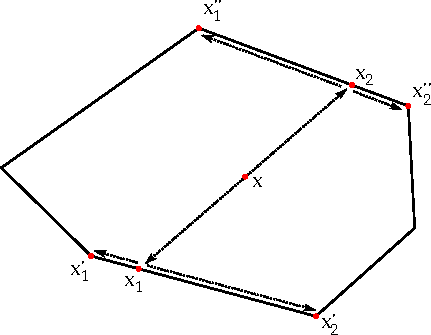
\includegraphics{./images/convex_comb_extr_points.pdf}
\end{center}
\caption{$x$ can be written as a convex combination of $x_1',x_2', x_1''$ and $x_2''$}
\label{Fig:convCombExPoints}
\end{figure}

Such an $\epsilon$ has to exist, since the polyhedron is bounded and therefore every line eventually crosses a boundary.\footnote{The calculation we did in the lecture to find $\epsilon_{1,2}$ seems dubious to the authors. We'll investigate.} Choosing $\epsilon$ like this implies that some constraint $a_i$ in $D$ has to become active for $x_1$ and the same holds with a different $a_i$ for $x_2$. Moving in direction $\delta$ doesn't affect the constraints that already were active, since $\delta$ is in the kernel of $B$. So we increase the number of active constraints and can extend $B$ to 

\[\begin{pmatrix}B\\ a_i\end{pmatrix}\] 

The rank of the new $B$ has to be $k+1$ since $\delta$ was orthogonal to all the vectors in $B$, as $B\delta=0$ (and hence all vectors in $\text{span } B$), but it is not orthogonal to $a_i$, or we wouldn't have hit that constraint by moving in direction $\delta$.

We have now reduced the problem of finding extreme points to represent $x \in P$ to the problem of finding some for $x_1,x_2 \in P$. However we increased the number of active constraints for $x_1,x_2$ (in 2D: we moved them on an edge). This process can be repeated for $x_1$ and $x_2$ until the respective $B$ has full rank and we arrived at some extreme points. For figure \ref{Thm:CH_polyhedron} the process is repeated three times, for $x,x_1$ and $x_2$. 
Since all the points from the beginning can be recursively written by a convex combination of the new points and we end up at an extreme point, the original $x$ can transitively be written by a convex combination of extreme points.
\end{description}

% Ich hab noch drüber nachgedacht und die Rechnung da in der Tat komisch zu sein. Er (oder ich :D) scheint sich zwischendurch verrechnet zu haben. Wir haben nicht genug info das zu lösen:
%
% x&=\lambda x_1+(1-\lambda)x_2 % ist die Linie zwischen x1,2 auf der x liegt. Wir wollen x_1,2 soweit nach außen schieben dass wir am Rand ankommen
% x&=\lambda (x+\epsilon_1\delta) + (1-\lambda)(x-\epsilon_2\delta) % ist das selbe nochmal neu geschrieben. Jetzt wollen wir nach den epsilons auflösen ???
% x-\lambda x - (1-\lambda) x = \lambda \epsilon_1\delta + (1-\lambda)\epsilon_2\delta
% x -\lambda x - x +\lambda x  = \epsilon_1\delta +\epsilon_2\delta
% 0 = \epsilon_1 \delta + \epsilon_2\delta
% ???
% Profit.



%In particular choose \label{wieso}
%\begin{align*}
%x&=\lambda x_1+(1-\lambda)x_2\\
%&=x+\underbrace{\lambda \epsilon_1\delta -(1-\lambda)\epsilon_2\delta}_{\stackrel{!}{=}0}\\
%&\Rightarrow \lambda = \frac{\epsilon_2}{\epsilon_1+\epsilon_2}
%\end{align*}

\end{pr}

\begin{cor}\label{Cor:always_extreme_points} Let $P$ be a non-empty bounded polyhedron. Then the LP $\min cx$ s.t. $x\in P$ always has an optimal solution that is an extreme point of $P$.
\end{cor}

Intuitively this is true, as given an optimal solution, which is not an extreme point, we could always go into the direction of a constraint which is not tight. Such a constraint must exist, as otherwise we would be at an extreme point. 

\begin{pr}[Corollary \ref{Cor:always_extreme_points}] %(from the book 'Linear Optimization') 
Start with some optimal solution $x^*$. Write it as a convex combination of extreme points 
\[x^* = \sum_{i=1}^x \lambda_i y_i \qquad \text{s.t. } y_i \text{ is an extreme point}\]
We want to prove that there is an extreme point $y_i$ such that the cost $v$ are the same as in $x^{*}$, that is:

\[v = cx^* = cy_i\]

Obviously $cy_i\geq v$ since $x^*$ is an optimal solution. It can't be strictly greater for all $y_i$ or 
\[c\sum_{i=1}^x \lambda_i y_i \gneq v\]
since the $\lambda_i$ are greater than zero and $\sum_i \lambda_i =1$. %To see why observe this:
%
%\begin{align*}
%cx^* &= c\sum_{i} \lambda_i y_i\\
%&=\sum_i \lambda_i cy_i\\
%\intertex{assume $cy_i\gneq cx^*$}
%&< \sum_i \lambda_i cx^*\\
%\intertext{$\lambda_i$ sum to 1}
%&< cx^*
%\end{align*}
%
This would be a contradiction since $x^*=\sum_{i=1}^x \lambda_i y_i$. So there has to be at least one extreme point $y_i$ for which $cy_i=v$.
\end{pr}

Corollary \ref{Cor:always_extreme_points} gives us the nice result that we can transform the problem of optimising an LP to a discrete problem with finitely (albeit exponentially) many candidate solutions. This will of course be very useful in designing an algorithm for solving them.

\subsection*{Fourier-Motzkin elimination}

In this section we're interested in computing representations of projections of polyhedra. See figure \ref{Fig:polyhedron_proj} for an example.

\begin{figure}[hbt]
\begin{center}
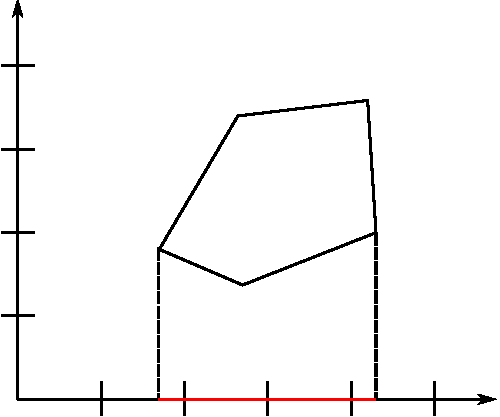
\includegraphics[width=0.3\textwidth]{./images/polyhedron_proj.pdf}
\end{center}
\caption{A projection which removes one of the two dimensions.}
\label{Fig:polyhedron_proj}
\end{figure}

\begin{Def} The projection $x=(\nthings{x})$ onto its first $k$ coordinates is $\pi_k(x) = (x_1,\ldots, x_k)$. 

Let $S\subseteq \R^n$ then the projection on the first $k$ components is

\[\pi_k(S)=\{\pi_k{x}|x\in S\}\]
\end{Def}

Of course that definition is not particularly useful in actually constructing the projection. The Fourier-Motzkin elimination computes the projection for polyhedra. We start with our usual characterisation of a polyhedron $P=\{x|Ax\geq b_i\}$ and want to find a different matrix $A'$ s.t. we get $\pi_{n-1}(P)$. Generalizing to $\pi_k$ is then of course easy.

\subsubsection*{Example of Fourier-Motzkin elimination}
Figure \ref{Fig:motzkinExample} shows an example of the Fourier-Motzkin elimination. The LP used for the example is:
\begin{eqnarray*}
c_1 & -0,5x + y & \leq 3 \\
c_2 & 2x + y & \leq 6 \\
c_3 & x+3y & \geq 6 \\
c_4 & x+y & \geq 2
\end{eqnarray*}
Those constraints can be rewritten to:
\begin{eqnarray*}
c_1 & \frac{1}{2}x + 3  & \geq y \\
c_2 & -2x+6 & \geq y \\
c_3 & y & \geq -\frac{1}{3}x+2 \\
c_4 & y & \geq -x+2
\end{eqnarray*}
Writing them this way has the advantage of ordering them around $y$. With this information we can build a new LP, which constraints are only on the x-dimension. The constraints are all the ordered pairs of around $y$.
\begin{eqnarray*}
c_1 \geq c_3: & \frac{1}{2}x + 3 & \geq -\frac{1}{3}x+2  \\
c_2 \geq c_3: & -2x+6 &  \geq -\frac{1}{3}x+2 \\
c_1 \geq c_4: & \frac{1}{2}x + 3   & \geq -\frac{1}{3}x+2 \\
c_2 \geq c_4: & -2x+6 & \geq -x+2
\end{eqnarray*}
Those constraints are shown in figure \ref{Fig:motzkinExample} below the x-axis with dashed lines. Note that we're only interested in the red part. So the two constraints $c_2 \geq c_3$ and $c_1 \geq c_4$ would be enough. As there is no efficient way to find those two constraints we have to keep all of them. 

\begin{figure}[hbt]
\begin{center}
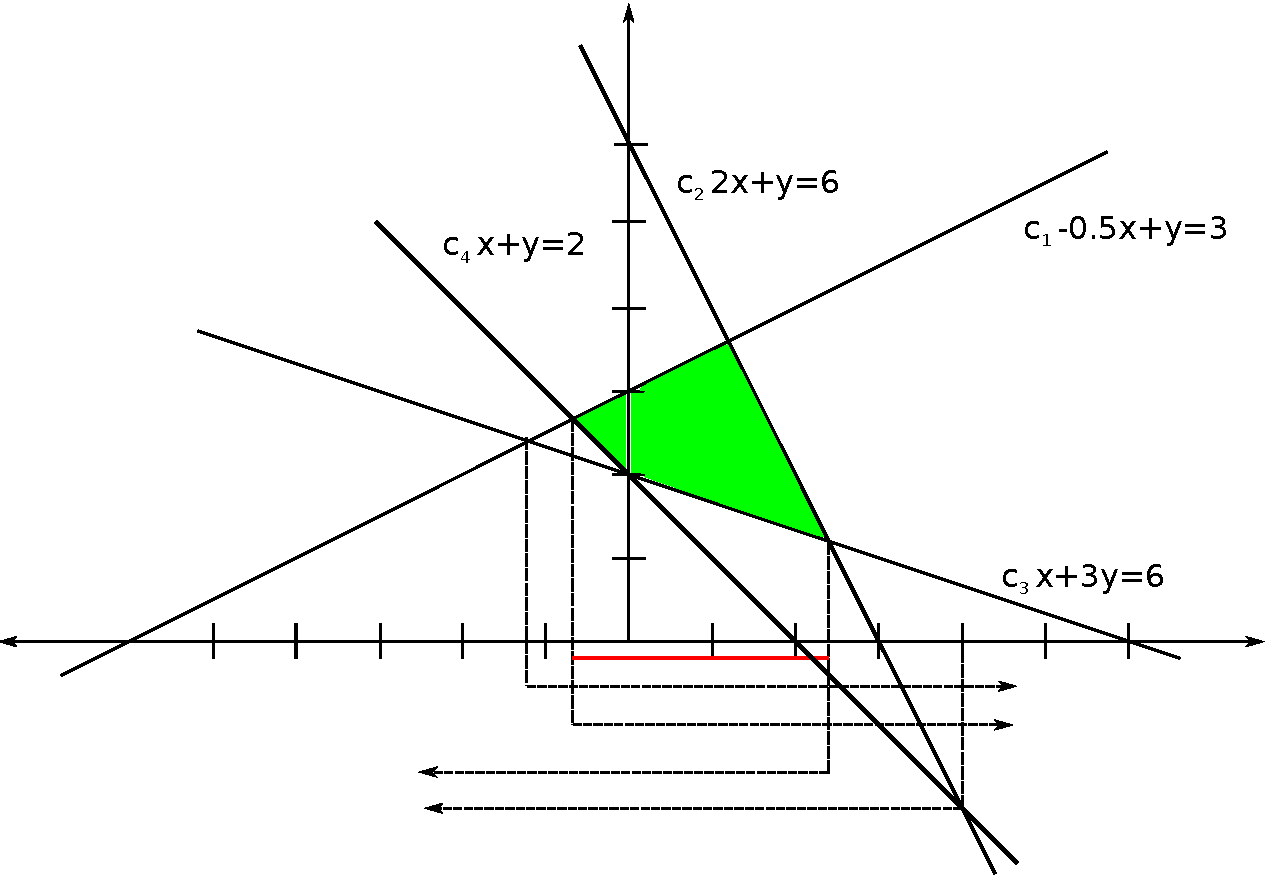
\includegraphics[width=0.8\textwidth]{./images/motzkin.pdf} %TODO die gestrichelten Linien mit c_1,..,4 beschriften 
\end{center}
\caption{A projection, which removes one of the two dimensions. The result is shown in red.}
\label{Fig:motzkinExample}
\end{figure}

\subsubsection*{General case}
We want to classify the constraints $a_i$ into three kinds. Let $\overline a = \pi_{n-1}(a)$ then we can write  

\[P=\left\{x\left| \begin{array}{cr}
\overline a_i\overline x +a_{in}x_n \geq b_i & i\in T_1\\
\overline a_i\overline x +a_{in}x_n \geq b_i & i\in T_2\\
\overline a_i\overline x \geq b_i & i\in T_3\\
\end{array}\right.\right\}\]

With 
$$\forall i\in T_1: a_{in}>0$$ $$\forall i\in T_2: a_{in}<0$$ $$ \forall i\in T_3: a_{in}=0 $$

From that form we rewrite the polyhedron by dividing by $\overline a_{in}$ if $\overline a_{in}\neq 0$. The $f_i$ are vectors and the $d_i$ are scalars. 

\begin{equation}\label{For:Motz1}x_n \geq  d_i + f_i \bar x : i \in T_1 \end{equation}
\begin{equation}\label{For:Motz2}x_n \leq  d_i+f_i \bar x : i \in T_2 \end{equation}
\begin{equation}\label{For:Motz3}0 \geq  d_i+f_i \bar x : i \in T_3 \end{equation}

%\[P \{i\in T_1 \wedge x_n \geq d_i + f_i \bar x \vee i\in T_2 \wedge x_n \leq d_i + f_i \bar x \vee i\in T_3 \wedge 0 \leq d_i + f_i \bar x\}\]

Then we can write the projection $\overline P=Q$ as\footnote{The lecture notes of both authors read: $\{d_i+f_i\bar x \leq d_j+f_j\bar x\ \forall i\in T_2, j\in T_1 $. The book says $\geq$ and $T_2\geq x_n \geq T_1$}

\begin{eqnarray*}
\{d_i+f_i\bar x & \geq d_j+f_j\bar x\ & \forall i\in T_2, j\in T_1  \\
d_i+f_i\bar x & \geq 0\ & \forall i\in T_3\}
\end{eqnarray*}

%$$\{d_i+f_i\bar x \geq d_j+f_j\bar x\ \forall i\in T_2, j\in T_1 $$ 
%$$d_i+f_i\bar x \geq 0\ \forall i\in T_3\}$$

Herein lies the problem of the algorithm. We introduce a new constraint for every pair of constraints from $T_1,T_2$. Hence in every iteration the number of constraints $c$ can grow on the order of $(\frac{c}{2})^2$.

\subsubsection*{Proof of correctness}
\begin{pr} To prove the correctness of the Fourier-Motzkin elimination we need to show that the result $Q$ of the algorithm is equal to $\pi_{n-1}(P)$. We do this by showing $\pi_{n-1}(P) \subset Q$ and $Q \subset \pi_{n-1}(P)$.
\begin{enumerate}

\item $\bar x \in \pi_{n-1}(P) \Rightarrow \bar x\in Q$. That means 
\[\exists x_n: \left[{\bar x}\atop{x_n}\right] \in P \Rightarrow {{\max_{i\in T_1} d_i +f_i \bar x \leq x_n} \atop {\min_{i\in T_2} d_i+fi\bar x \geq x_n}}\]
Therefore the constraints \ref{For:Motz1}, \ref{For:Motz2} and \ref{For:Motz3} are satisfied. It follows that $\bar x \in Q$. 

\item $\bar x \in Q \Rightarrow \bar x \in \pi_{n-1}(P)$. Choosing $x_n$ as 
\[x_n \in [\max_{i\in T_1} d_i+f_i \bar x, \min_{i\in T_2} d_i+f_i \bar x]\]
does the trick, as $(\bar x, x)$ then satisfies constrains \ref{For:Motz1}, \ref{For:Motz2} and \ref{For:Motz3} and therefore is in $P$.

\end{enumerate}
\end{pr}

There are a lot of interesting applications for these projections:

\begin{thm}\label{Thm:linTransPoly} Let $P\in \R^n$ be a polyhedron and $A\in \R^{m\times n}$ be a matrix. Then the set
\[Q=\{Ax|x\in P\}\]
is also a polyhedron.
\end{thm}

In 2D this is intuitively clear: applying linear transformations on polygons results in distorted, rotated etc. polygons. For higher dimensions it follows from the projections:

\begin{pr}[Theorem \ref{Thm:linTransPoly}] For $P$ we have

\[Q=\{(Ax,x)\in \R^{m+n}| x\in P, P\text{ is a polyhedron in } \R^{n}, A \in \R^{m \times n}\}\]  %this is actually not that intuitive for me. Why is this a polyhedron?

is a polyhedron. Then $\pi_m(Q)$ is also a polyhedron.
\end{pr}

\begin{cor} Let $x_1,x_2,\ldots, x_k \in \R^n$, then CH($x_1,x_2,\ldots, x_k$) is a polyhedron\end{cor}

\paragraph*{Optimal value} We can use the projections to find the optimal value for an LP (not the optimal solution though). Suppose we're given a LP in the usual form, $\min cx$ s.t. $Ax\geq b$. We construct the following polyhedron P:

\begin{eqnarray*}
 & (x_0,\ldots,x_n) & \\
s.t. & A(x_0,\ldots,x_n)^{\mbox{T}} & \geq b \\
& c(x_0,\ldots,x_n)^{\mbox{T}} & = x_0
\end{eqnarray*}

Define $Q = \pi_1(P)$. We can find $Q$ with the Fourier-Motzkin elimination. If $Q$ is not feasible, $P$ is empty. Else we can choose the biggest $b_i$ such that $x_0\geq b_i$ or the smallest $b_i$ such that $x_0 \leq b_i$, depending on the type of constraints we have. That is the optimal value.

\begin{thm}[Farkas' lemma] Let $A\in \R^{m\times n}$ and $b\in \R^m$. Then either 
\begin{itemize}
\item $\exists x\in \R^n: Ax\geq b$ or
\item $\exists y\in \R^m, y\geq 0, y^{\mbox{T}}A=0: y\cdot b>0$
\end{itemize}
\end{thm} 

This theorem is very nice if we want to check if some system of inequalities is feasible. We just have to find the vector $y$. This lemma can be proven by our earlier results. (Sketch:) We start with the polygon $P$ and use a projection to get rid of the last dimension of $P$. By that we get another matrix $B$ and another vector $d$. We get the new inequalities by combining those from the original polyhedron. Instead of actually doing the projection to a lower dimension we can replace the last element by 0. You can show that $[B0]=DA$ (no proof). You can repeat that process until you get a matrix $F$ such that $FA=0$. The system is infeasible if you end up with a negative rhs for a constraint, since all lhs will be 0.